\documentclass[a4paper, 12pt]{article}		% general format

%%%% Charset
\usepackage{cmap}							% make PDF files searchable and copyable
\usepackage[utf8x]{inputenc}				% accept different input encodings
\usepackage[T2A]{fontenc}					% Russian font
\usepackage[russian]{babel}					% multilingual support (T2A)

%%%% Graphics
\usepackage[dvipsnames]{xcolor}			% driver-independent color extensions
\usepackage{graphicx}						% enhanced support for graphics
\usepackage{wrapfig}						% produces figures which text can flow around

%%%% Math
\usepackage{amsmath}						% American Mathematical Society (AMS) math facilities
\usepackage{amsfonts}						% fonts from the AMS
\usepackage{amssymb}						% additional math symbols

%%%% Typography (don't forget about cm-super)
\usepackage{microtype}						% subliminal refinements towards typographical perfection
\linespread{1.3}							% line spacing
\usepackage[left=2.5cm, right=1.5cm, top=2.5cm, bottom=2.5cm]{geometry}
\setlength{\parindent}{0pt}					% we don't want any paragraph indentation
\usepackage{parskip}						% add distance between paragraphs

%%%% Tables
\usepackage{tabularx}						% Normal tables
\usepackage{multirow}						% for tabular
\usepackage{hhline}							% for tabular


%%%% Other
\usepackage{url}							% verbatim with URL-sensitive line breaks
\usepackage{fancyvrb}						% verbatim with box
\setcounter{secnumdepth}{5}					%

%------------------------------------------------------------------------------
\usepackage{listings}						% typeset source code listings

% Настройки отображения кода
\lstset{
	% Настройки отображения
	breaklines=true,						% Перенос длинных строк
	basicstyle=\ttfamily\footnotesize,		% Шрифт для отображения кода
	frame=tblr								% draw a frame at all sides of the code block
	tabsize=2,								% tab space width
	showstringspaces=false,					% don't mark spaces in strings
	% Настройка отображения номеров строк. Если не нужно, то удалите весь блок
	numbers=left,							% Слева отображаются номера строк
	stepnumber=1,							% Каждую строку нумеровать
	numbersep=5pt,							% Отступ от кода
	numberstyle=\small\color{black},		% Стиль написания номеров строк
}

% Для настройки заголовка кода
\usepackage{caption}
\renewcommand{\lstlistingname}{Листинг} % Переименование Listings в нужное именование структуры
%------------------------------------------------------------------------------
\author{Семён Мартынов\\<semen.martynov@gmail.com>}
\title{Отчет по лабораторной работе 3:\\AirCrack}
\begin{document}
\maketitle
\tableofcontents{}

%------------------------------------------------------------------------------

\newpage
\section{Набор инструментов для аудита беспроводных сетей AirCrack}

\subsection{Цель работы}

Изучить основные возможности пакета AirCrack и принципы взлома WPA/WPA2 PSK и WEP.

\subsection{Ход работы}

\subsubsection{подготовка испытательного стенда}

Для проведения данной работы использовалась специально подготовленная WiFi-сеть, параметры которой представлены на рисунке 1.

\begin{figure}[h!]
\centering
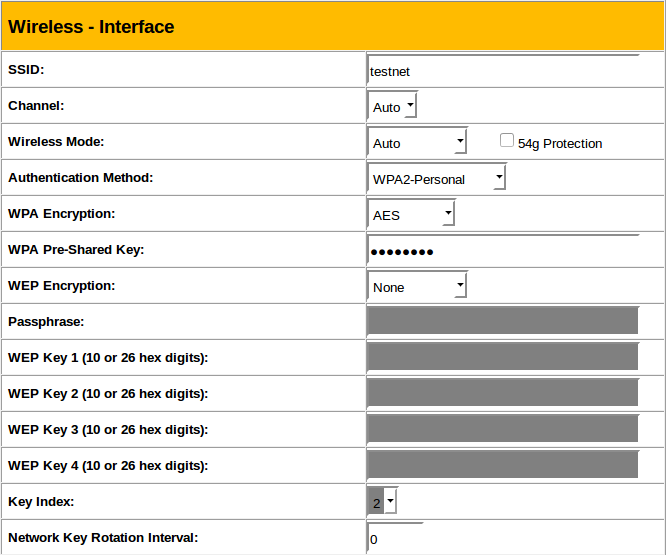
\includegraphics[scale=0.45]{res/pic01}
\caption{Параметры сети}
\end{figure}

Пароль выбран исходя из требований web-интерфейса роутера - он содержит не менее 7 символ, включая спецсимволы.

Утилиты из набора AirCrack запускались из дистрибутива BlackArch, т.к. Kali linux (вернее Debian) имеет проблему с поддержкой драйверов современных устройств. Скриншоты в BlackArch делать неудобно, поэтому в отчёте будет приведён текстовый вывод консоли.

\subsubsection{Запуск режима мониторинга на беспроводном интерфейсе}

Этот режим позволяет адаптеру видеть весь беспроводной трафик (вернее не отбрасывать не свои пакеты), который ему физически доступен. Команда и ей вывод показаны в листинге 1.

\lstinputlisting[firstline=0,lastline=7,language={},caption={Запуск режима мониторинга}]{res/log.txt}

\subsubsection{Сбор трафика}

Команда airodump-ng позволяет захватить весь физически доступный трафик и распознать имена сетей, каналы, точки доступа и клиентов. В листинге 2 с 5-й по 30-ю строки перечислены точки доступа, а с 30-й по 48-ю клиенты.

\lstinputlisting[firstline=8,lastline=56,language={},caption={Весь трафик}]{res/log.txt}

В 8-й строчке можно видеть нашу целевую сеть; её BSSID 00:23:54:A1:CE:17 и она работает на 8-м канале. Теперь можно запустить airodump-ng с параметрами отслеживания именно этой сети (листинг 3). Параметр \textit{--write} обеспечивает запись трафика в файл с префиксом dump.

\lstinputlisting[firstline=57,lastline=69,language={},caption={Отслеживание сети testnet}]{res/log.txt}

\subsubsection{Деаутентификация прочих клиентов}

Для захвата зашифрованного пароля нужно иметь клиентскую аутентификацию на точке доступа. Если пользователь уже прошел проверку подлинности, то можно его деаутентифицировать и тогда система автоматически повторит аутентификацию, и в этот момент можно перехватить нужный пакет.

В листинге 4 показано, как используя знания о физическом адресе клиента, мы (в отдельном окне терминала) делаем 10 попыток деаутентификации. Можно было отправить и широковещательный запрос, но некоторые современные точки доступа имеют защиту от такого трюка.

\lstinputlisting[firstline=71,lastline=85,language={},caption={Деаутентификация клиентов}]{res/log.txt}

В это время, в окне сбора трафика, в правом верхнем углу появляется сообщение \textit{WPA handshake}, т.е. нужный пакет пойман (листинг 5).

\lstinputlisting[firstline=90,lastline=98,language={},caption={WPA handshake}]{res/log.txt}


\subsubsection{Взлом с использованием словаря паролей}

Когда зашифрованный пароль получен и сохранён в файл dump-01.cap, можно запустить aircrack-ng с базой распространённых паролей (листинг 6). В таких ситуациях, эксперты любят напоминать, что успешность атаки сильно зависит от качеств словаря паролей.
В нашем случае пароль был найден очень быстро.

\lstinputlisting[firstline=102,language={},caption={WPA handshake}]{res/log.txt}

\subsubsection{Взлом сети WEP}

Взлом WEP сети выполняется ещё проще, в том смысле, что небезопасность протокола даёт некоторые гарантии взломщику. 

Проблема заложено в самой архитектуре -- шифрование потока осуществляется при помощи временного ключа. Вместе с каждым пакетом данных  WEP передаёт несколько байт этого самого ключа. Таким образом, вне зависимости от сложности ключа раскрыть любую передачу можно просто имея достаточное число перехваченных пакетов (10 000 пакетов мне всегда хватало, что довольно мало для активно использующейся сети).

Не смотря на крайне низкую степень безопасности, этот протокол до сих пор можно встретить, что видно в листинге 2.

\newpage
\subsection{Выводы}

Обеспечить безопасность беспроводной сети довольно сложно. В данный момент наиболее распространены сети с защитой wep2, но, как мы убедились в этой работе, для них требуются достаточно длинные и сложные (не словарные) пароли. Новые дыры в безопасности создаёт WPS ( который часто включен по умолчанию на многих SoHo роутерах), ошибки в прошивках роутеров (с бекдорами и уязвимым софтом) и вирусы (которые похищают реквизиты доступа к роутеру из списка сохранённых паролей в браузере).

%------------------------------------------------------------------------------

\end{document}
